\documentclass[tikz,border=8pt]{standalone}
\usepackage{amsmath}
\usetikzlibrary{arrows.meta,positioning,fit,calc}

\begin{document}
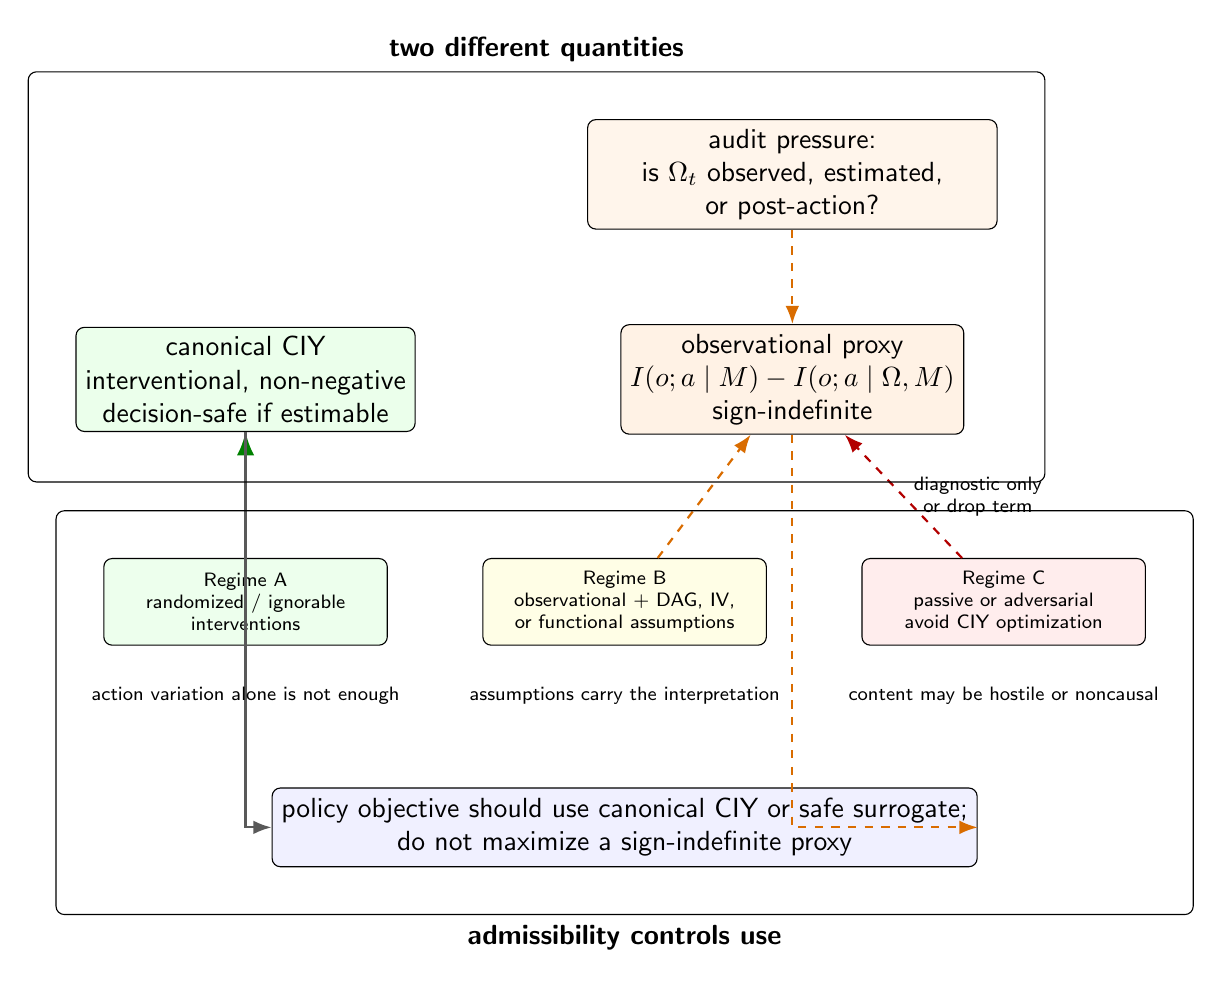
\begin{tikzpicture}[
  font=\sffamily,
  box/.style={draw, rounded corners=3pt, align=center, minimum width=40mm, minimum height=10mm, fill=white},
  regime/.style={draw, rounded corners=3pt, align=center, minimum width=36mm, minimum height=11mm, fill=white, font=\sffamily\scriptsize},
  arrow/.style={-Latex, thick, draw=black!65},
  good/.style={-Latex, very thick, draw=green!50!black},
  warn/.style={-Latex, thick, dashed, draw=orange!85!black},
  bad/.style={-Latex, thick, dashed, draw=red!70!black},
  note/.style={align=center, font=\sffamily\scriptsize}
]

\node[box, fill=green!8] (canon) {canonical CIY\\interventional, non-negative\\decision-safe if estimable};
\node[box, right=26mm of canon, fill=orange!10] (proxy)
  {observational proxy\\$I(o;a\mid M)-I(o;a\mid\Omega,M)$\\sign-indefinite};

\node[regime, below=16mm of canon, fill=green!7] (a)
  {Regime A\\randomized / ignorable\\interventions};
\node[regime, right=12mm of a, fill=yellow!10] (b)
  {Regime B\\observational + DAG, IV,\\or functional assumptions};
\node[regime, right=12mm of b, fill=red!7] (c)
  {Regime C\\passive or adversarial\\avoid CIY optimization};

\draw[good] (a) -- (canon);
\draw[warn] (b) -- (proxy);
\draw[bad] (c) -- node[right, note] {diagnostic only\\or drop term} (proxy);

\node[box, below=18mm of b, fill=blue!6, minimum width=78mm] (safe)
  {policy objective should use canonical CIY or safe surrogate;\\do not maximize a sign-indefinite proxy};
\draw[arrow] (canon) |- (safe);
\draw[warn] (proxy) |- (safe);

\node[box, above=12mm of proxy, fill=orange!8, minimum width=52mm] (omega)
  {audit pressure:\\is $\Omega_t$ observed, estimated,\\or post-action?};
\draw[warn] (omega) -- (proxy);

\node[note, below=4mm of a] {action variation alone is not enough};
\node[note, below=4mm of b] {assumptions carry the interpretation};
\node[note, below=4mm of c] {content may be hostile or noncausal};

\node[draw, rounded corners=3pt, fit=(canon)(proxy)(omega), inner sep=6mm,
  label={[font=\sffamily\bfseries]above:two different quantities}] {};
\node[draw, rounded corners=3pt, fit=(a)(b)(c)(safe), inner sep=6mm,
  label={[font=\sffamily\bfseries]below:admissibility controls use}] {};

\end{tikzpicture}
\end{document}
